% SIAM Article Template
\documentclass[review,onefignum,onetabnum]{siamonline181217}

% Information that is shared between the article and the supplement
% (title and author information, macros, packages, etc.) goes into
% ex_shared.tex. If there is no supplement, this file can be included
% directly.

% SIAM Shared Information Template
% This is information that is shared between the main document and any
% supplement. If no supplement is required, then this information can
% be included directly in the main document.


% Packages and macros go here
\usepackage{lipsum}
\usepackage{amsfonts}
\usepackage{graphicx}
\usepackage{epstopdf}
\usepackage{algorithmic}
\ifpdf
  \DeclareGraphicsExtensions{.eps,.pdf,.png,.jpg}
\else
  \DeclareGraphicsExtensions{.eps}
\fi

\graphicspath{{./Figures/}}

% Prevent itemized lists from running into the left margin inside theorems and proofs
\usepackage{enumitem}
\setlist[enumerate]{leftmargin=.5in}
\setlist[itemize]{leftmargin=.5in}

% Add a serial/Oxford comma by default.
\newcommand{\creflastconjunction}{, and~}

% Used for creating new theorem and remark environments
\newsiamremark{remark}{Remark}
\newsiamremark{hypothesis}{Hypothesis}
\crefname{hypothesis}{Hypothesis}{Hypotheses}
\newsiamthm{claim}{Claim}
\newsiamthm{prop}{Proposition}

% Sets running headers as well as PDF title and authors
\headers{Bayesian inversion of a diffusion model with application to Biology}{J.-C. Croix, N. Durrande, and M. A. \'Alvarez}

% Title. If the supplement option is on, then "Supplementary Material"
% is automatically inserted before the title.
\title{Bayesian inversion of a diffusion model with application to Biology\thanks{Submitted to the editors DATE.
\funding{This work has been supported by Colciencias and ECOS-Nord under the grant C15M04}}}

% Authors: full names plus addresses.
\author{Jean-Charles Croix\thanks{School of Mathematical and Physical Sciences, University of Sussex, Falmer, UK 
  (\email{j.croix@sussex.ac.uk}).}
\and Nicolas Durrande\thanks{Prowler.io, Cambridge, UK 
  (\email{nicolas@prowler.io}).}
\and Mauricio A. \'Alvarez\thanks{Department of Computer Science, University of Sheffield, UK 
  (\email{mauricio.alvarez@sheffield.ac.uk}).}}

\usepackage{amsopn}
\DeclareMathOperator{\diag}{diag}

%\usepackage{float}

%%% Local Variables: 
%%% mode:latex
%%% TeX-master: "ex_article"
%%% End: 


% Optional PDF information
\ifpdf
\hypersetup{
  pdftitle={Bayesian inversion of a diffusion model with application to Biology},
  pdfauthor={J.-C. Croix, N. Durrande, and M. A. \'Alvarez}
}
\fi

% The next statement enables references to information in the
% supplement. See the xr-hyperref package for details.

%\externaldocument{ex_supplement}

% FundRef data to be entered by SIAM
%<funding-group specific-use="FundRef">
%<award-group>
%<funding-source>
%<named-content content-type="funder-name"> 
%</named-content> 
%<named-content content-type="funder-identifier"> 
%</named-content>
%</funding-source>
%<award-id> </award-id>
%</award-group>
%</funding-group>

\begin{document}

\maketitle

% REQUIRED
\begin{abstract}
  A common task in experimental sciences is to fit mathematical models to real-world measurements to improve understanding of natural phenomenon (reverse-engineering or inverse modelling). When complex dynamical systems are considered, such as partial differential equations, this task may become challenging or ill-posed. In this work, a linear parabolic equation is considered as a model for protein transcription from MRNA. The objective is to estimate jointly the differential operator coefficients, namely the rates of diffusion and self-regulation, as well as a functional source. The recent Bayesian methodology for infinite dimensional inverse problems is applied, providing a unique posterior distribution on the parameter space continuous in the data. This posterior is then summarized using a Maximum a Posteriori estimator. Finally, the theoretical solution is illustrated using a state-of-the-art MCMC algorithm adapted to this non-Gaussian setting.
\end{abstract}

% REQUIRED
\begin{keywords}
  Bayesian Inverse Problems, Diffusion equation, Functional MCMC, Gaussian processes.
\end{keywords}

% REQUIRED
\begin{AMS}
  62G05, 62P10, 35R30, 62F15
\end{AMS}

\section{Introduction}

The problem of diffusion in a porous media, which is ubiquitous in Physics, Engineering and Biology, is usually represented by the following partial differential equation (with constant diffusion and damping without transport):
\begin{equation}
\begin{aligned}
\frac{\partial z}{\partial t}(x,t)+\lambda z(x,t)-D\Delta z(x,t)&=f(x,t),\;\forall(x,t)\in\Omega\times]0,T],\\
z(x,t)&=0,\;\forall (x,t)\in\Omega\times\lbrace t=0\rbrace,\\
z(x,t)&=0,\;\forall (x,t)\in\partial\Omega\times]0,T].\\
\end{aligned}
\label{eq:PDE}
\end{equation}
where the spatial domain is an open set $\Omega\subset\mathbb{R}^n$ ($n\leq 3$) and the final time is $T\in\mathbb{R}^+$ (other initial and boundary conditions are possible). In real world applications, the quantity of interest $z$ (hereafter called the solution of equation \ref{eq:PDE}) is typically the concentration of some chemical and evolves from a null initial state under three distinct mechanisms: a) direct variation in concentration, given by the source $f$, b) diffusion at rate $D$, c) production or depletion at a rate $\lambda$. Different hypotheses on the parameters lead to a well-defined solution (well-posedness in the sense of Hadamard) but only a particular case will be dealt with here. Besides the traditional computation of the solution from the parameters, one can use this model for the determination of an optimal control (e.g. source leading to the minimization of a particular cost functional) or the identification of parameters from partial knowledge of the solution in an inverse setting and the latter is the objective of this paper. The motivation comes from a challenging identification problem in Biology where the objective is to infer jointly self-regulation and diffusion rates with the source $f$ given a limited number of noisy observations of the solution $z$. Note that given their physical interpretation, the parameters $u=(\lambda,D,f)$ must all be non-negative (in an obvious sense).
\newline
\newline
This problem has already been solved by different approaches, using different models. In \cite{Becker2013}, the authors use a system of ordinary differential equations instead of equation \ref{eq:PDE}, and minimize a discrete version of a least-square penalty functional, while confidence intervals on parameters are given by bootstrapping. In a Bayesian setting, alternative methods have been based on Latent Force Models \cite{Alvarez2013,Sarkka2017}. These approaches assume that the source can be modelled with Gaussian Processes \cite{Rasmussen2006}. In particular, if $f$ is such process and if the decay and the diffusion are constants, $z$ is Gaussian as well (since $z$ depends linearly in $f$). The two constant parameters $\lambda$ and $D$ can then be optimized as hyper-parameters through standard likelihood maximization. Major drawbacks of this approach are both the difficulty to enforce positiveness of the reconstructed source and the absence of uncertainty quantification on $\lambda,D$.
\newline
\newline
In this work, a more general methodology is applied, based on the recent advent of Bayesian Inverse Problems \cite{Stuart2010} for infinite dimensional spaces. This has the advantage of dealing with the ill-posedness while fully integrating the quantification of uncertainties in a unified approach. Moreover, the possibility to include previous physical constraints in the prior will be particularly meaningful. The rest of this paper is organized as follows: \cref{sec:BayesianInv} presents all the mathematical analysis underlying the Bayesian inversion, namely sufficient regularity of the forward operator (mapping the parameter $(\lambda,D,f)$ to the PDE solution $z$), existence and uniqueness of the posterior under a simple class of priors,and finally uniqueness of the associated posterior. \cref{sec:MCMCsampling} focuses on an adaptation of a geometric Markov Chain Monte-Carlo algorithm, well-defined in function spaces. Finally, \cref{sec:NumericalExperiments} contains all implementation details, as well as a methodology to tune hyper-parameters of the model. All numerical results are based on a real-world dataset related to the developmental biology of the Drosophila Melanogaster.

\section{Bayesian inversion}
\label{sec:BayesianInv}

As previously announced, the goal in this work is to infer a source term $f$ (mRNA concentration) jointly with rates of diffusion $D$ and decay $\lambda$ (i.e. the parameter $u=(\lambda,D,f)$) from noisy and partial measurements of the solution $z$ (gap protein concentration). This problem is ill-posed for multiple reasons: a) the parameter $u$ is infinite dimensional and only finite data are available, b) the solution map is not injective and c) observations are noisy. The typical approach to alleviate this issue is to regularize the problem, usually adding more constraints with Tikhonov-Philips functionals, to ensure uniqueness and continuity w.r.t. the observations \cite{Isakov2017, Schuster2012}. Doing so, the regularized solution will be compatible with the dataset, but possibly very different from the \emph{real} parameter (if there is such thing). Additionally, a particularly valuable information is a representation of all parameters $u$ that would lead to similar data, giving precise statement on how the dataset is informative \cite{Ghanem2017, Biegler2011, Sullivan2015}. One approach consists in treating these 2 objectives sequentially, first regularizing then quantifying the resulting uncertainty. However, the Bayesian methodology for inverse problems (\cite{Stuart2010} and more recently \cite{Dashti}) is precisely tailored to complete both tasks at once in an elegant manner. One particularity of these recent contributions is to tackle inverse problems directly in function spaces, postponing discretization at the very end for implementation purposes, which leads to robust algorithms w.r.t. discretization dimension. Indeed, finite approximations of probability measures may be absolutely continuous while their infinite counterparts are mutually singular. This becomes particularly troublesome in MCMC sampling for instance \cite{Cotter2013}.
\newline
\newline
In essence, instead of searching for one particular parameter solving the regularized problem, this approach considers conditional probability measures of parameters given observations. Namely, given a prior distribution (see \cref{sec:ChoicePrior}) and few technical conditions on the forward operator (see \cref{sec:ForwardModel}), Bayes theorem applies and exhibits a unique posterior distribution (see \cref{sec:PosteriorDistribution}), which is continuous in the data (w.r.t. Hellinger metric). Finally, one may summarize information from this posterior distribution with point estimators such as expected value or modes (\cref{sec:MAP}). All these steps will now be presented.

\subsection{Forward model analysis}
\label{sec:ForwardModel}

The first step is to detail precisely the required regularity of the solution map from equation \ref{eq:PDE}. Using common variational techniques from PDE theory (see \cite{Evans1998} or \cite{Brezis2011}), one can show that this equation has a unique weak solution (see \cref{prop:SolutionOperator} which proof is in the appendix) given $u=(\lambda,D,f)$ in a domain $\mathcal{U}$ that will be precised later on. Moreover, this solution evolves smoothly when the parameter varies. Without any loss of generality and keeping in mind the Biological application, the underlying physical domain will be $\Omega=]0,L[$ with $L\in\mathbb{R}^+$, representing the anterior-posterior axis of a Drosophilia embryo.

\begin{prop}
	Let $0<\lambda_M$, $0<D_m\leq D_M$, $\mathcal{U}=[0,\lambda_M]\times[D_m,D_M]\times \mathcal{C}([0,T]\times[0,L];\mathbb{R})$ with the norm $ \lVert u\rVert_{\mathcal{U}}=\vert\lambda\vert+\vert D\vert+\lVert f\rVert_{\infty}$, then for all $u\in\mathcal{U}$, equation \ref{eq:PDE} has a unique weak solution $z$, continuous on the domain $[0,L]\times [0,T]$, defining the map:
	\begin{equation*}
	z:u\in \mathcal{\mathcal{U}}\to z(u)\in C([0,T]\times[0,L];\mathbb{R}).
	\end{equation*}
	Moreover, this map has the following properties:
	\begin{enumerate}
		\item (Energy estimate): it satisfies the following estimate $\forall u\in\mathcal{U}$,
		\begin{equation*}
		\lVert z(u)\rVert_{\infty}\leq C\lVert f\rVert_{\infty},
		\end{equation*}
		where $C>0$ is a constant independent of $u$,
		\item (Local Lipschitz continuity): $\forall u$ in the interior of $\mathcal{U}$, $\forall r>0$ such that $\mathcal{B}(u,r)\subset\mathcal{U}$, $\exists L(u,r)>0$,
		\begin{equation*}
		\forall (u_1,u_2)\in\mathcal{B}(u,r)\times\mathcal{B}(u,r),\;\lVert z(u_1)-z(u_2)\rVert_{\infty}\leq L(u,r)\lVert u_1-u_2\rVert_{\mathcal{U}}
		\end{equation*}
		\item (Differentiability): it is twice Fr\'echet differentiable in the interior of $\mathcal{U}$.
	\end{enumerate}
	\label{prop:SolutionOperator}
\end{prop}

The proof is standard using methods from PDE and optimal control theory \cite{Evans1998}. The properties stated in \cref{prop:SolutionOperator} will be important for subsequent analysis (\cref{sec:PosteriorDistribution}):
\begin{enumerate}
	\item The energy estimate is fundamental to establish most of the results concerning the posterior distribution. Indeed, it gives a precise upper bound, useful to show integrability of the yet-to-come likelihood,
	\item Local Lipschitz continuity implies measurability of the solution map w.r.t. the Borel $\sigma$-algebra and is used in the characterization of posterior modes (Maximum a Posteriori estimators),
	\item Second order Fr\'echet differentiability will be necessary for geometric methods in optimization (research of posterior modes) and sampling (Markov-Chain Monte-Carlo) since they rely on Hessian-type information.
\end{enumerate}

\subsection{Choice of a prior distribution}
\label{sec:ChoicePrior}

The second step is to choose a prior probability distribution on $\mathcal{U}$, encoding all knowledge on the problem at hand, while being simple enough to keep analysis tractable. The prior will be constructed as a product measure, specifying individual measures $\mu_0^\lambda$, $\mu_0^D$, $\mu_0^f$ on all parameters first, thus:
\begin{equation}
\mu_0(du):=\mu_0^\lambda(d\lambda)\otimes\mu_0^D(dD)\otimes\mu_0^f(df).
\label{eq:PriorMeasure}
\end{equation}
For simplicity, both measures for $\lambda$ and $D$ will be taken uniform on respective intervals $[D_m,D_M]$ and $[0,\lambda_M]$. Now, since $f$ must be non-negative, \ref{eq:PDE} is re-parametrized with the following source term:
\begin{equation}
f^*=\exp(f),
\label{eq:Reparametrization}
\end{equation}
where $f\in C([0,T]\times[0,L];\mathbb{R})$. Now, selecting a Borel probability measure $\mu_0^f$ on $C([0,T]\times[0,L];\mathbb{R})$ will imply both continuity and positivity almost-surely of the new source $f^*$. The energy estimate is adjusted:
\begin{equation*}
\forall u\in\mathcal{U},\;\lVert z(u)\rVert_{\infty}\leq C^*\exp\left(\lVert f\rVert_{\infty}\right).
\end{equation*}
In this work, $\mu^f_0$ will be taken as the Gaussian measure associated with a continuous Gaussian process (see \cite{Bogachev1998} for a presentation of infinite dimensional Gaussian measures) such that $f$ is almost-surely continuous. Remark that the exponential map in equation \ref{eq:Reparametrization} could be replaced with any sufficiently differentiable function from $\mathbb{R}$ to $\mathbb{R}^+$ (thus keeping the second order Fr\'echet differentiability of the solution map). Besides, alternative distributions are also possible for $f$ like Besov priors (from \cite{Dashti2013}) or more general convex measures from \cite{Hosseini2017a}. However, this choice is also motivated by practical reasons, since one can find a Gaussian measure $\mu_{ref}$ dominating $\mu_0$:
\begin{equation*}
\mu_{ref}=\mathcal{N}(\lambda_{ref},\sigma_\lambda^2)\otimes\mathcal{N}(D_{ref},\sigma_D^2)\otimes\mu_0^f.
\label{eq:GaussianRef}
\end{equation*}
Indeed, choose $(\lambda_{ref},D_{ref})\in\mathbb{R}^2$ and $\sigma_\lambda^2,\sigma_D^2>0$ then $\mu_0<<\mu_{ref}$ with
\begin{equation*}
\frac{d\mu_0}{d\mu_{ref}}(u)=\frac{d\mu_0^\lambda}{d\mu_{ref}^\lambda}(\lambda)\frac{d\mu_0^D}{d\mu_{ref}^D}(D)=\frac{2\pi\sigma_\lambda\sigma_D}{\lambda_M(D_M-D_m)}\exp\left(\frac{(\lambda-\lambda_{ref})^2}{2\sigma_\lambda^2}+\frac{(D-D_{ref})^2}{2\sigma_D^2}\right).
\label{eq:RNdensityRef}
\end{equation*}
The parameters of $\mu_{ref}$ are tuned by choosing $\lambda_{ref}=\frac{\lambda_M}{2}$, $\sigma_\lambda^2=\frac{\lambda_M^2}{12}$, $D_{ref}=\frac{D_M-D_m}{2}$ and $\sigma_D^2=\frac{(D_M-D_m)^2}{12}$ (minimizing Kullback-Leibler divergence of $\mu_{ref}$ relative to $\mu_0$). This dominant measure will be critical for posterior modes analysis (section \ref{sec:MAP}) and MCMC sampling (section \ref{sec:MarkovKernel}). 

\subsection{Posterior distribution}
\label{sec:PosteriorDistribution}

It is now time to show that the particular setting provided so far (forward model and prior distribution) leads to a well defined posterior measure. This is the purpose of \cref{prop:PosteriorMeasure} which is a direct application of the theory initially developed in \cite{Stuart2010} (see \cite{Dashti} for an updated presentation). In this purpose, consider a dataset $y=(y_i)_{i\in[1,n]}\in\mathbb{R}^n$ consisting of observations from the solution $z$ at different times and locations $(t_i,x_i)_{i\in[1,n]}\in\left([0,T]\times[0,L]\right)^n$, produced under the following additive noise model (in vector notations):
\begin{equation}
y=\mathcal{G}(u)+\eta,
\label{eq:ObservationModel}
\end{equation}
where $\eta\sim\mathcal{N}(0,\sigma_\eta^2I_n)$ ($I_n$ being the identity matrix of dimension $n$) and $\mathcal{G}:\mathcal{U}\to\mathbb{R}^n$ is the observation operator, mapping directly the PDE parameter $u$ to the value of the associated solution $(z[u](x_i,t_i))_{i\in[1,n]}$ (composition of solution map $z$ with Dirac type measure). Note that it is well-defined since the function $z$ is continuous on the domain for every $u\in\mathcal{U}$. The following proposition, which is again proved in the appendix, establishes the existence, uniqueness and continuity in $y$ of the posterior probability measure $\mu^y$ (the solution of the inverse problem), expressing how observations $y$ updated prior beliefs $\mu_0$ on the parameter $u$.
\begin{prop}
	Let $\mathcal{G}$ be the observation operator defined in equation \ref{eq:ObservationModel}, $y\in\mathbb{R}^n$ a dataset and $\mu_0$ the probability measure defined in equation \ref{eq:PriorMeasure}, then there exists a unique posterior measure $\mu^y$ for $u\vert y$. It is characterized by the following Radon-Nikodym density w.r.t. $\mu_0$:
	\begin{equation*}
	\forall u\in\mathcal{U},\;\frac{d \mu^y}{d\mu_0}(u)=\frac{1}{Z(y)}\exp\left(-\Phi(u;y)\right),
	\end{equation*}
	with the negative log-likelihood
	\begin{equation*}
	\Phi(u;y)=\frac{1}{2\sigma_\eta^2}\lVert y-\mathcal{G}(u)\rVert_{\mathbb{R}^n}^2,
	\end{equation*}
	and the marginal
	\begin{equation*}
	Z(y)=\int_\mathcal{U}\exp(-\Phi(u;y)\mu_0(du).
	\end{equation*}
	Furthermore, $\mu^y$ is continuous in $y$ w.r.t. Hellinger distance.
	\label{prop:PosteriorMeasure}
\end{prop}
In fact, proposition \ref{prop:PosteriorMeasure} gives two distinct results: a) the existence and uniqueness of a posterior (as long as $\mu_0$ is Radon and $\mu_0(\mathcal{U})=1$, which is the case here), b) well-posedness of the Bayesian inverse problem. In particular, the use of a Gaussian prior on $f$ gives sufficient integrability, even under the re-parametrization from equation \ref{eq:Reparametrization} (using Fernique's theorem). If one chooses a different map between $f^*$ and $f$, this condition may be considerably relaxed (using a square map for instance) and prior measures with lower integrability conditions can be considered.

\subsection{Maximum a posteriori}
\label{sec:MAP}

In the previous section, the well-posedness of the Bayesian inverse problem has been proved. However, the posterior distribution is only known up to a multiplicative constant, through its density w.r.t. $\mu_0$. In the application, $\mu^y$ will need to be summarized, which is usually done by the selection of a particular estimator in $\mathcal{U}$, such the posterior mean or a mode. One consequence of \cref{prop:PosteriorMeasure} is that the posterior mean is automatically continuous in the data $y$ (since well-posedness is w.r.t. Hellinger distance, see \cite{Dashti}). However, optimality properties (in a decision theoretic context) are not yet well-understood in infinite dimension to the best of our knowledge. This is why posterior modes (or Maximum a Posteriori) are considered instead. Furthermore, they provide a clear link with the classical Tikhonov-Philips regularization (see \cite{Dashti2013,Helin2015,Agapiou2018}) and a useful variational characterization (in case of Gaussian or Besov priors) which will be the cornerstone of the numerical application, see \cref{prop:MAP} (which proof is given in the appendix).

\begin{prop}
	Let $\mu_0$ be the prior probability measure defined in equation \ref{eq:PriorMeasure} and $\mu_{ref}$ the Gaussian reference measure from equation \ref{eq:RNdensityRef}, then the modes of $\mu^y$ are exactly the minimizers of the following (generalized) Onsager-Machlup functional:
	\begin{equation*}
	I(u):=\Phi(u;z)+\frac{1}{2}\lVert f\rVert^2_{\mu_0^f},
	\label{eq:Onsager}
	\end{equation*}
	where $\lVert.\rVert_{\mu_0^f}$ is the Cameron-Martin norm associated to $\mu_0^f$.
	\label{prop:MAP}
\end{prop}

A minimizer of the previous generalized Onsager-Machlup functional will be noted $u_{MAP}=(\lambda_{MAP},D_{MAP},f_{MAP})$ and need not be unique. The precise application of this proposition to the biological setting is done in \cref{sec:ChoiceOfPriors}, once the prior distribution is fully specified.

\subsection{Approximation}

The final step in the theoretical analysis of the Bayesian inverse problem is to study its approximation properties, since it will be solved numerically. There are two important things to check: a) properties of the approximated posteriors (since it is what is available), b) the consistency of these approximated posteriors. This will be done by projection of the parameter $u$ onto a finite dimensional subspace of $\mathcal{U}$, constructed with a stochastic basis under $\mu_0^f$ (see \cite{Okazaki1986} for a detailed introduction on stochastic bases including Banach spaces). The second source of approximation is the use of a numerical solver for the PDE solution, but this will be neglected here (but can be conducted in a subsequent work). The next proposition will establish that the posterior distribution is well approximated, giving an estimate of the error when the Hilbert basis is chosen specifically (spectral basis of the covariance operator, namely Karhunen-Lo\`eve decomposition) and its proof is in the appendix.

\begin{prop}
	Let $\mu_0$ be the prior probability measure from \ref{eq:PriorMeasure}, $\mathcal{G}$ the observation operator from equation \ref{eq:ObservationModel}, $y\in\mathbb{R}^n$ a dataset, $(f_n)_{n\in\mathbb{N}}\subset\mathcal{C}([0,L]\times[0,T];\mathbb{R})$ a stochastic basis for $\mu^0_f$. Note $\forall m \in\mathbb{N}$, $P_mf$ the projection of $f$ onto the span of $f_1,\dots,f_m$ and $(\Phi_m)_{m\in\mathbb{N}}$ the following sequence of approximate negative log-likelihoods:
	\begin{equation*}
	\Phi_m(u;y):=\Phi((\lambda,D,P_mf);y),
	\end{equation*}
	then the sequence $(\Phi_m)_{m\in\mathbb{N}}$ defines a family of posterior measures $(\mu_m^y)_{m\in\mathbb{N}}$, all continuous w.r.t. $y$ and such that
	\begin{equation*}
	\lim_{m\to\infty}d_{Hell}(\mu^y,\mu^y_m)=0.
	\end{equation*}
	\label{prop:Approximation}
\end{prop}

\section{Metropolis-Hastings algorithm}
\label{sec:MCMCsampling}

As it was previously announced, the main motivation for the Bayesian methodology here is quantification of uncertainty, which will be done by sampling the posterior measure. Among the vast catalogue of methods for probability distributions simulation (Sequential Monte-Carlo, Approximate Bayesian Computations, Transport Maps, etc...), Markov chain Monte-Carlo is very popular (MCMC, see \cite{Brooks2011}) and well defined on function spaces \cite{Tierney1998} even though ergodicity analysis of such algorithms is still in its infancy \cite{Hairer2005,Hairer2007,Hairer2014,Rudolf2018}. After a short presentation of the Metropolis-Hastings algorithm (\cref{sec:MH}), this section will focus on a state-of-the-art Markov kernel designed to sample from Gaussian measures (\cref{sec:MarkovKernel}) and adapt it to the current non-Gaussian prior using the Gaussian dominating measure $\mu_{ref}$.

\subsection{Metropolis-Hastings on function spaces}
\label{sec:MH}

The Metropolis-Hastings algorithm (MH) is a very general \cite{Tierney1998} method to design Markov chains to sample from a given probability measure. It is based on a two-step process on each iteration:
\begin{enumerate}
	\item Given a current state $u\in\mathcal{U}$, propose a new candidate $v$ according to a proposal Markov kernel $Q(u,dv)$ (it is a probability distribution on $\mathcal{U}$ for almost any $u\in\mathcal{U}$),
	\item Accept the new state $v$ with probability $\alpha(u,v)$ or remain at $u$.
\end{enumerate}
This algorithm provides a sample distributed under a predefined probability measure $\mu$, if one selects $\alpha$ and $Q$ in a specific way (see \cite{Tierney1998} for a discussion in general state spaces). For instance, let $\nu(du,dv)=\mu(du)Q(u,dv)$ and $\nu^T(du,dv)=\nu(dv,du)$, the Metropolis-Hastings algorithm typically considers the following acceptance probability:
\begin{equation}
\alpha_{MH}(u,v)=\min\left(1, \frac{d\nu^T}{d\nu}(u,v)\right),
\end{equation}
which, in particular, requires the absolute continuity of $\nu^T$ w.r.t. $\nu$ (detailed balance condition of the Markov chain). Contrary to finite dimensional situations, this condition may be difficult to satisfy and a common way to overcome this situation in Bayesian Inverse problems (see \cite{Dashti,Girolami2011,Beskos2017a,Cotter2013,Hairer2014}) is to select $Q$ revertible w.r.t. $\mu_0$. Indeed, in this case (with $\nu_0(du,dv)=\mu_0(du)Q(u,dv)$):
\begin{equation}
\frac{d\nu^T}{d\nu}(u,v)=\frac{\frac{d\nu^T}{d\nu^T_0}(u,v)}{\frac{d\nu}{d\nu_0}(u,v)}=\frac{\frac{d\mu^y}{d\mu_0}(v)}{\frac{d\mu^y}{d\mu_0}(u)}=\exp\left(\Phi(u;y)-\Phi(v;y)\right).
\label{eq:Acceptance}
\end{equation}
In theory, the MH algorithm can be implemented with a large family of proposal kernels $Q$. In practice however, they need to be as efficient as possible and thus adapted to the problem at hand. Two common desirable properties for $Q$ are:
\begin{itemize}
	\item to adjust to locally mimic the target distribution $\mu^y$,
	\item include a step size to tune acceptance probability to reasonable values.
\end{itemize}
These two properties may be used to trade-off self-correlation, acceptance rates and convergence speed to high interest areas of the parameter space. Next section presents a proposal $Q$ with both properties to sample from a Gaussian prior distribution.

\subsection{Geometric MCMC under Gaussian reference}
\label{sec:MarkovKernel}

The specific Markov proposal kernel $Q$, tailored to sample distributions having a density w.r.t. a Gaussian measure $\mu_{ref}$ will now be presented. Most of the recent work on infinite dimensional MCMC methods are based on the following Langevin stochastic differential equation:
\begin{equation}
\frac{du}{dt}=-\frac{1}{2}K(u)\left(\mathcal{C}_{ref}^{-1}(u-u_{ref})+\nabla_u\Phi(u;y)\right)+\sqrt{K(u)}\frac{dW}{dt},
\label{eq:Langevin}
\end{equation}
where $K(u)$ is a (possibly position-dependent) preconditioner, $W$ a cylindrical Brownian motion and $\nabla_u\Phi(u;y)$ the gradient in $u$ of the negative log-likelihood. According to \cite{Beskos2017a}, a semi-implicit discretization of equation \ref{eq:Langevin} leads to a Markov chain with the following kernel:
\begin{equation}
Q(u,dv)=\mathcal{N}\left(\rho (u-u_{ref})+u_{ref}+\sqrt{1-\rho^2}\frac{\sqrt{h}}{2}g(u),\sqrt{1-\rho^2}K(u)\right),
\label{eq:MarkovKernel}
\end{equation}
where $h>0$ is a step-size parameter, $\rho=\frac{1-h}{1+h}$ and:
\begin{equation*}
g(u)=-K(u)\left[(\mathcal{C}_{ref}^{-1}-K(u)^{-1})(u-u_{ref})+\nabla_u\Phi(u;y)\right].
\end{equation*}
This dynamic explores the parameter space with a balance between Newton-type descent to zones of high density and Gaussian exploration. The philosophy behind this kernel is to use alternative Gaussian reference measures locally adapted to the posterior distribution, since it has been recently showed that higher efficiency is obtained from operator weighted proposals (\cite{Law2014} and later generalized in \cite{Beskos2017a} and \cite{Cui2016b}). Indeed, highly informative datasets may result in a posterior measure significantly different from the prior in likelihood-informed directions and non-geometric kernels (such as Independent sampler or preconditioned Crank-Nicholson for instance) become ineffective in this case. However, the infinite dimensional manifold Modified Adjusted Langevin Algorithm ($\infty$-mMALA from \cite{Beskos2017a}) considers a specific preconditioner:
\begin{equation*}
K(u)=\left(\mathcal{C}_{ref}^{-1}+H_\Phi(u)\right)^{-1},
\end{equation*}
where $H_\Phi(u)$ is the Gauss-Newton Hessian operator of $\Phi$, which locally adapts to the posterior. This kernel does not preserve the distribution $\mu^y$ but is shown to be absolutely continuous w.r.t. the reference measure $\mu_{ref}$, almost-surely in $u$ (under technical assumptions regarding $K(u)$ linked with Feldman-Hajek theorem) and the Radon-Nikodym density is:
\begin{equation*}
\frac{dQ(u,dv)}{d\mu_{ref}}(v)=\frac{dN\left(\frac{\sqrt{h}}{2}g(u),K(u)\right)}{dN(0,\mathcal{C})}\left(\frac{v-\rho (u-u_{ref})-u_{ref}}{\sqrt{1-\rho^2}}\right),
\end{equation*}
and noting $w=\frac{v-\rho (u-u_{ref})-u_{ref}}{\sqrt{1-\rho^2}}$ as it is done in \cite{Beskos2017a}, it finally comes:
\begin{equation*}
\begin{split}
\ln\left(\frac{dQ(u,dv)}{d\mu_{ref}}(u,v)\right)
&=-\frac{h}{8}\vert K(u)^{-\frac{1}{2}}g(u)\vert^2
+\frac{\sqrt{h}}{2}\langle K(u)^{-\frac{1}{2}}g(u),K(u)^{-\frac{1}{2}}w\rangle\\
&-\frac{1}{2}\langle w,H_\Phi(u)w\rangle+ln\left(\left\vert\mathcal{C}_{ref}^{\frac{1}{2}}K(u)^{-\frac{1}{2}}\right\vert\right).
\end{split}
\end{equation*}
Finally, the acceptance probability associated to the Markov kernel from equation \ref{eq:MarkovKernel} is
\begin{equation*}
\alpha(u,v)=\min\left(1,\frac{\frac{dQ}{d\mu_{ref}}(v,u)\frac{d\mu^y}{d\mu_0}(v)}{\frac{dQ}{d\mu_{ref}}(u,v)\frac{d\mu^y}{d\mu_0}(u)}\right).
\end{equation*}
This algorithm is well-defined on function spaces (reversibility is ensured w.r.t. $\mu_0$), thus it is robust to discretization as required. The $\infty$-mMALA proposal may be computationally expensive, as it requires to compute both gradient $\nabla\Phi$, Gauss-Newton Hessian $H_\Phi$ and the Cholesky decomposition of $K(u)^{-1}$ at each step. However, different dimension reduction techniques can be used (split in \cite{Beskos2017a} or likelihood-informed in \cite{Cui2016b}) to reduce the computational burden. A second alternative is to choose a constant preconditioner, located at a (precomputed) posterior mode for instance (similar to HMALA in \cite{Cui2016b} and gpCN in \cite{Rudolf2018}), which is done in this work.

\section{Numerical application}
\label{sec:NumericalExperiments}

This section will now introduce the practical implementation of the previous methodology on the problem of reverse-engineering for post-transcriptional gap-gene in Drosophila Melanogaster. First, the prior distribution is detailed, as well as a random series representation for $f$, leading to an approximation of $f^*$. Moreover, the associated generalized Onsager-Machlup functional is also provided. Then, quantitative results are given on the dataset taken from \cite{Becker2013}, consisting in protein concentration measurements irregularly spread in space and time.

\subsection{Choice of a continuous Gaussian process}
\label{sec:ChoiceOfPriors}

In the previous analysis, $\mu_0^f$ has been defined as the probability measure over $\mathcal{C}([0,L]\times[0,T];\mathbb{R})$ associated with a continuous Gaussian process. In practice, it will be chosen centred for simplicity, thus completely specified by a covariance kernel over the space-time domain $[0,L]\times [0,T]$. The literature on such processes is vast (see \cite{Rasmussen2006} for instance), and here a tensor product of two Brownian bridges (in time and space) will be used. The associated covariance kernel is given by:
\begin{equation}
	K((x,t),(x',t'))=\sigma^2\frac{4}{LT}\left(\min(x,x')-\frac{xx'}{L}\right)\left(\min(t,t')-\frac{tt'}{T}\right),
\end{equation}
where the scaling constant is such that the process has maximum variance equal to $\sigma^2$. In particular, this process has a well-known Karhunen-Loeve decomposition (see \cite{Bay2017}) using Schauder-type hat functions. In turn, the process will thus be approximated as follows:
\begin{equation}
\begin{split}
\tilde{f}&=\sum_{1\leq i_1,i_2\leq N}\sigma\sqrt{\lambda_{i_1,i_2}}\xi_i\varphi_{i_1,i_2},\\
\varphi_{i_1,i_2}(x,t)&=\varphi_{i_1}\left(\frac{x}{L}\right)\varphi_{i_2}\left(\frac{t}{T}\right),\;\forall (x,t)\in[0,L]\times[0,T],\\
\lambda_{i_1,i_2}&=\lambda_{i_1}\lambda_{i_2},
\end{split}
\end{equation}
where $(\xi_{i_1,i_2})_{1\leq i_1,i_2\leq N}$ are i.i.d. $\mathcal{N}(0,1)$ random variables and $\varphi_{i}$ are hat functions on dyadic intervals and the precise weights are given in \cite{Bay2017}. We consider $N=20$ (400 basis functions) thus the approximated parameter $\tilde{u}=(\lambda,D,\tilde{f})$ is of dimension 402.

\subsection{Solution map discretization}
\label{sec:Discretization}

The analysis conducted in all previous sections happens to be valid for infinite dimensional quantities. In practice however, one needs to discretize for numerical experiments. In this work, the solution map is approximated using finite elements in space (FEniCS library in Python, see \cite{Alnae2015} and \cite{Langtangen2017}) and finite differences in time. We use 100 finite elements and 30 time steps on a 2018 standard laptop computer\footnote{All codes are available online at \url{https://github.com/JeanCharlesCroix/2019_Bayesian_Melanogaster}.}. We set $L=100$ and $T=100$ is the final time (data-points have been rescaled). All quantities related to negative log-likelihood derivatives (Gradient and Gauss-Newton Hessian matrix) are numerically computed using discrete adjoint methods (see \cite{Hinze2009} or \cite{Heinkenschloss2008}) to keep scalability in $N$. The initial point in the chain is chosen at the MAP location, obtained by minimization of the functional in equation \ref{eq:Onsager} (Prior based initialization results in long burnin phase). Practical optimization is done using L-BFGS-B algorithm from the Scipy library \cite{Byrd1995}.

\subsection{Estimation of noise variance}

So far, the prior measure as well as the observation model include hyper-parameters playing fundamental roles and needing to be tuned. The complete list is $\lambda_M,D_m,D_M,\sigma_\eta^2$ and to the best of our knowledge, there are no general methods to estimate them efficiently in this context. Indeed, no closed formulae exists for the likelihood (probability density of $\mathcal{G}(u)$) and cross-validation seems computationally out of reach. However, we provide here an empirical approach to tune the noise variance level $\sigma^2_\eta$. The other parameters are fixed to arbitrary values. Our approach consists in:
\begin{enumerate}
	\item Fix $\hat{\sigma}_\eta^2=1$.
	\item Find $u_{MAP}$ minimizing $I$ using the current noise level $\sigma_\eta^2$.
	\item Update the current variance estimation $\hat{\sigma}_\eta^2=\frac{1}{n-1}\lVert y-\mathcal{G}(u_{MAP})\rVert^2$.
	\item Go back to $2$.
\end{enumerate}
The algorithm is stopped once the parameter $\sigma_\eta^2$ reach a stable value, which in this application is $\hat{\sigma}_\eta^2=20,50$. The estimator $u_{MAP}$ is taken as the last computed minimizer of the (discretized) Onsager-Machlup functional $I$.

\subsection{Results}
\label{sec:Melanogaster}

We now turn to our main objective, the inversion and uncertainty quantification of gap-gene protein concentration from \cite{Becker2013}. The dataset consists of 508 different measures which are non-uniformly spread in time and space (precise repartition can be seen in \cref{fig_MAPpost}). With this estimated value, we compute our initial MAP estimate (numerical minimization of the Onsager-Machlup functional) and use it as initial point in the MCMC sampling.
\begin{figure}[h!]
	\centering
	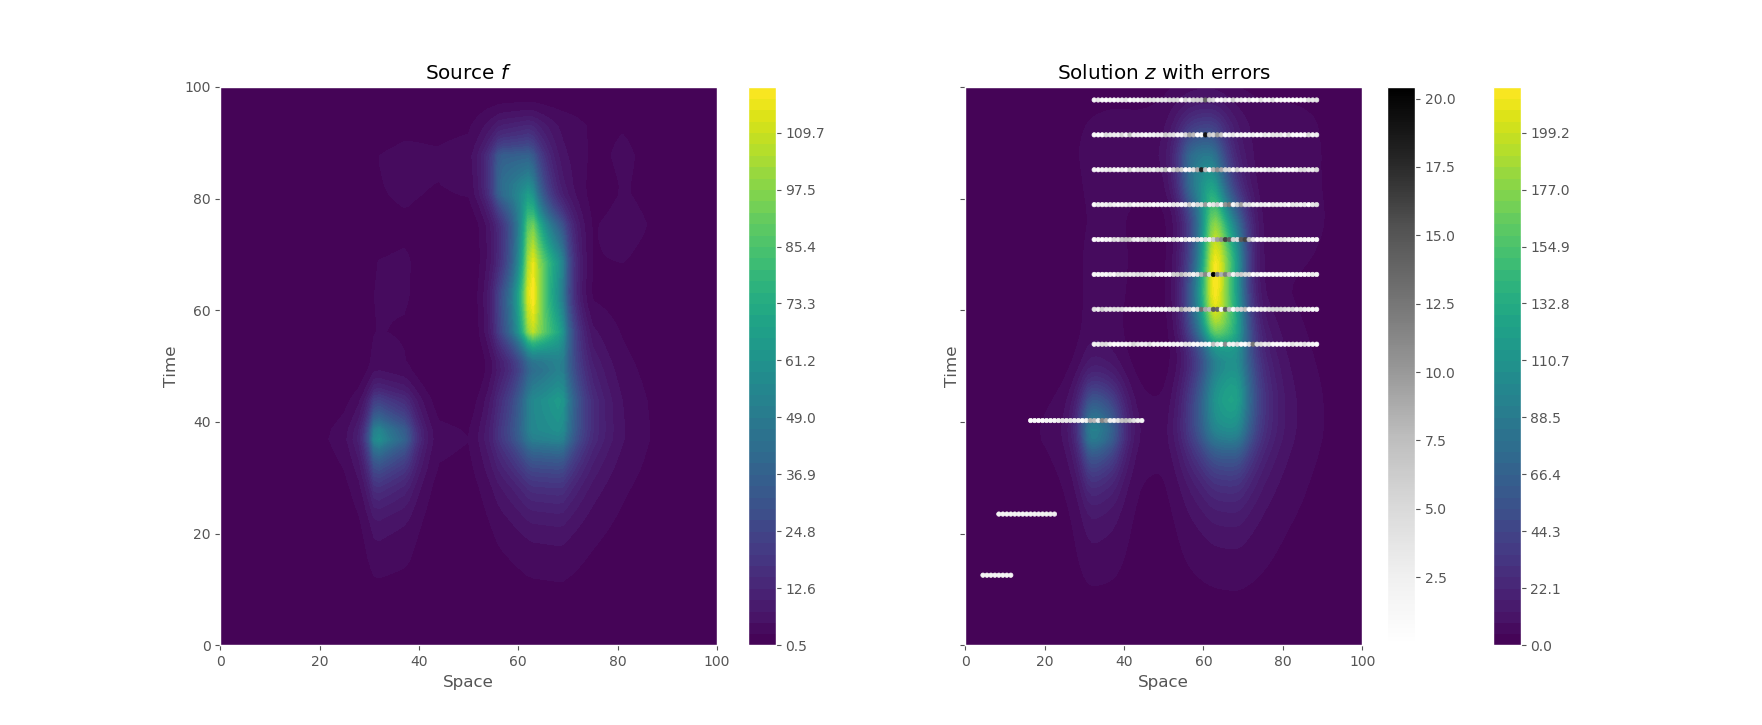
\includegraphics[width=1.0\linewidth]{MAP}
	\caption{MAP estimator $u_{MAP}$ from direct optimisation of the Onsager-Machlup functional. Left: Estimated source term $f_{MAP}$ (using 400 basis functions). Right: estimated solution $z(u_{MAP})$ with absolute error at data locations. Grey bar represents the level of error between $y$ and $\mathcal{G}(u_{MAP})$.}
	\label{fig_MAPpost}
\end{figure}
The Markov chain is ran for $21000$ total iterations and the resulting traceplot is given in \cref{fig_traceplot} for negative log-likelihood, decay, diffusion and first three components of $f$. The first thousand iterations are used as burnin and according to the autocorrelation function (\cref{fig_acf}), we choose to keep one iteration out of two hundreds as posterior sample (thinning). From this, we compute both posterior mean and MAP estimates, the precise values of decay, diffusion, negative log-likelihood and Onsager-Machlup functional being given in table \ref{table_estimates}.
\begin{table}[h!]
	\centering
	\begin{tabular}{c|c|c|c|c}
		Parameter & $\lambda$ & $D$ & $\Phi(u;z)$ & $I(u)$ \\
		\hline
		MAP (optimisation) & $0.47$ & $0.62$ & $254.54$ & $416.47$ \\ 
		Posterior Mean (sampling) & $0.47$ & $0.69$ & $253.28$ & $419.29$\\
	\end{tabular}
	\caption{Values of decay, diffusion, negative log-likelihood and Onsager-Machlup functional for MAP and posterior mean estimators.}
	\label{table_estimates}
\end{table}
Additionally to the estimated values, one can also look at the marginal distribution on \cref{fig_scatter}.
\begin{figure}[h!]
	\centering
	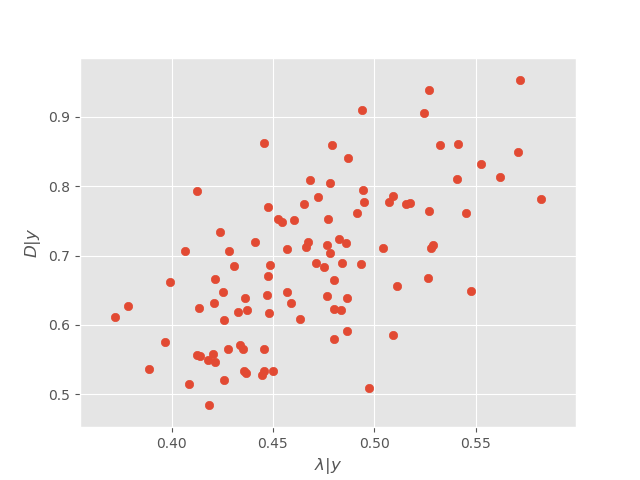
\includegraphics[width=0.8\linewidth]{Scatter}
	\caption{Marginal posterior distributions for $\lambda\vert y$ and $D\vert y$.}
	\label{fig_scatter}
\end{figure}
Concerning the MAP estimator (\cref{fig_MAPpost}), we recover both events described in \cite{Becker2013}, that is 2 pikes of protein concentrations. The first happens on the anterior part of the embryo in the early experiment $(x=35,t=35)$. The second is much more intense and happens in the posterior part during the second half of the experiment. The estimated source explains these with an intense and localized increase in concentration. Finally, the uncertainty on both source and solution around data seems to be really low, which provides a good confidence on the level of mRNA at this time and part of the embryo (see \cref{fig_var}). However, the point-wise variance on the solution $y$ remains important before the first observations, which translates an expected level of uncertainty.
\begin{figure}[h!]
	\centering
	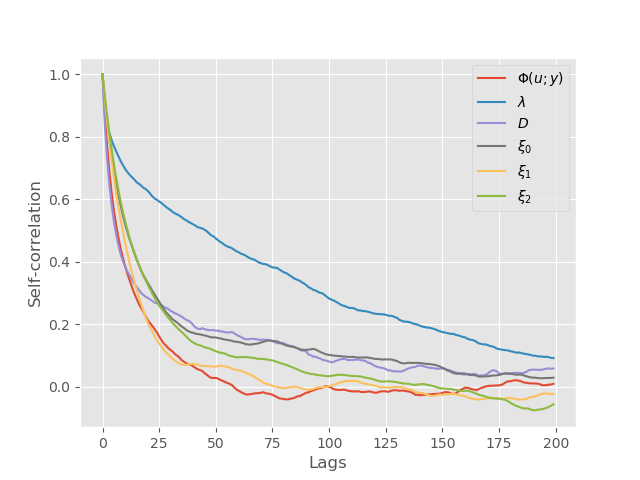
\includegraphics[width=0.8\linewidth]{Acf}
	\caption{Self-correlation of $\Phi(u;y)$, $\lambda$, $D$, $\xi_0$, $\xi_1$ and $\xi_2$, excluding the first 1000 iterations.}
	\label{fig_acf}
\end{figure}

\begin{figure}[h!]
	\centering
	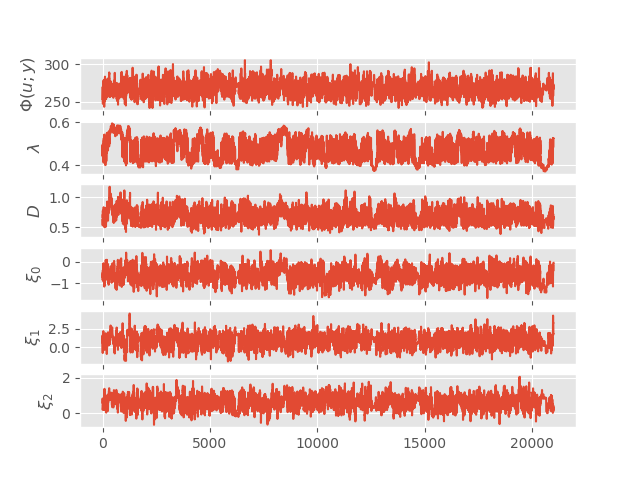
\includegraphics[width=0.8\linewidth]{Trace}
	\caption{Trace plots of $\Phi(u;y)$, $\lambda$, $D$, $\xi_0$, $\xi_1$ and $\xi_2$ (the first 1000 iterations are burned).}
	\label{fig_traceplot}
\end{figure}

\begin{figure}[h!]
	\centering
	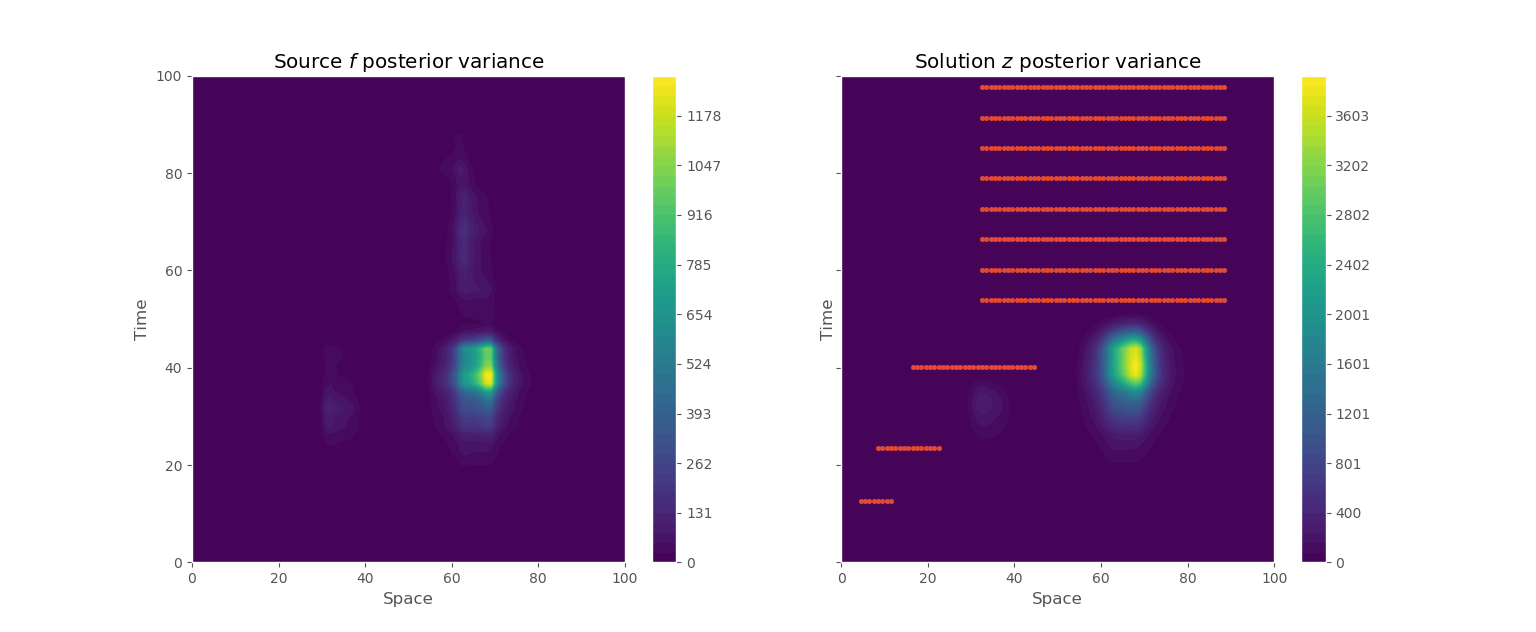
\includegraphics[width=1.0\linewidth]{Variance}
	\caption{Posterior point-wise variance of $f^*\vert y$ (left figure) and $z(u)\vert y$ (right figure).}
	\label{fig_var}
\end{figure}

\section{Conclusions}
\label{sec:conclusions}

In this work, we applied the Bayesian inverse problem methodology from \cite{Stuart2010} to a practical Biological dynamical system. Doing so, we provide a rigorous and detailed analysis of the forward model, existence and continuity of the posterior measure, characterization of maximum a posteriori (MAP) estimates, a consistent approximation and apply a state-of-the-art MCMC methodology. Because the forward MAP is non-linear, the uniqueness of posterior modes is unclear and it appears that local maximas are present. Nevertheless, the Bayesian methodology provides both a regularized solution to the problem, while giving a precious quantification of uncertainty. However, the estimation of prior hyper-parameters is still out of reach, giving poor confidence in the estimated variance. This direction requires further research, that we intend to address in a future work.

\appendix
\section{Proofs}

\begin{proof}[Proof of \cref{prop:SolutionOperator}]
	Using standard notations from PDE theory, let $\Omega=]0,L[$, $H=L^2(\Omega)$, $V=H^1_0(\Omega)$, $V^*=H^{-1}(\Omega)$ and
	\begin{equation*}
		W=\left\lbrace z\in L^2([0,T],V),\;z'\in L^2([0,T],V^*)\right\rbrace,
	\end{equation*}
	equipped with the norm:
	\begin{equation}
	\lVert z\rVert_{W}=\left(\lVert z\rVert^2_{L^2([0,T],V)}+\lVert z'\rVert^2_{L^2([0,T],V^*)}\right)^{\frac{1}{2}}
	\end{equation}
	\begin{enumerate}
		\item (Existence, uniqueness and energy estimate) Let $\mathcal{U}=[0,\lambda_M]\times[D_m,D_M]\times \mathcal{C}([0,T]\times[0,L])$ with $\lambda_M>0$ and $0<D_m\leq D_M<\infty$, then the differential operator in equation \ref{eq:PDE} is uniformly parabolic. By standard techniques, e.g. Galerkin approximation, one can show the existence and uniqueness of a weak solution $w\in W$ to equation \ref{eq:PDE} (Theorems 3 and 4, section 7.1, \cite{Evans1998}). Moreover, the regularity of the source term implies an improved regularity for the weak solution, namely $z\in L^2([0,T],H^2(\Omega))$ with $z'\in L^2([0,T],H)$ (Theorem 5, section 7.1, \cite{Evans1998}). The last result is an energy estimate:
		\begin{equation}
			\lVert z\rVert_{L^2([0,T],H^2(\Omega))}+\lVert z'\rVert_{L^2([0,T],H)}\leq C\lVert f\rVert_{L^2([0,T]\times[0,L])}.
		\end{equation}
		This in turn implies the announced energy estimate, by the two continuous embeddings: $L^2([0,T]\times[0,L])$ in $\mathcal{C}([0,T]\times[0,L])$ and $z$ into $\mathcal{C}([0,T]\times[0,L])$ (Theorem 4, section 5.9, \cite{Evans1998}):
		\begin{equation}
		\lVert z\rVert_{\infty}\leq C'\lVert f\rVert_{\infty}.
		\end{equation}
		\item (Local Lipschitz continuity in $u$, weaker norm) Let $u$ in the interior of $\mathcal{U}$, $r>0$ such that $\mathcal{B}(u,r)\subset\mathcal{U}$ and $(u_1,u_2)\in\mathcal{B}(u,r)\times\mathcal{B}(u,r)$. There exists two unique solutions with respect to $u_1$ and $u_2$ such that $\forall i\in\lbrace 1,2\rbrace$, $\forall v\in L^2([0,T],V)$ and for almost-every $t$ in $[0,T]$:
		\begin{equation*}
			\langle z_i'(t),v(t)\rangle_{V^*,V}+\lambda_i\langle z_i(t),v(t)\rangle_{H}+D_i\langle z_i(t),v(t)\rangle_{V}=\langle f_i(t),v(t)\rangle_{V^*,V},
		\end{equation*}
		which, using subtraction and rearranging the terms, leads to:
		\begin{equation}
		\begin{split}
		&\langle z_1'(t)-z_2'(t),v(t)\rangle_{V^*,V}+\lambda_1\langle z_1(t)-z_2(t),v(t)\rangle_{H}+D_1\langle z_1(t)-z_2(t),v(t)\rangle_{V}\\
		&=\langle f_1(t)-f_2(t),v(t)\rangle_{V^*,V}+(\lambda_2-\lambda_1)\langle z_2(t),v(t)\rangle_{H}+(D_2-D_1)\langle z_2(t),v(t)\rangle_{V}.
		\end{split}
		\label{ch5_eq_estimationv}
		\end{equation}
		Now, let $v=z_1-z_2$ in equation \ref{ch5_eq_estimationv}, drop the term $\lambda_1\lVert z_1-z_2\rVert_H^2$ in the left-hand side, use Cauchy-Schwarz and Poincar\'e's inequalities in the right-hand side, then:
		\begin{equation*}
			\begin{split}
				&\langle z_1'(t)-z_2'(t),z_1(t)-z_2(t)\rangle_{V^*,V}+D_1\lVert z_1(t)-z_2(t)\rVert^2_{V}\\
				&\leq
				\left(\lVert f_1-f_2\rVert_{V^*}+c\vert \lambda_2-\lambda_1\vert\lVert z_2\rVert_V+\vert D_2-D_1\vert\lVert z_2\rVert_{V}\right)\lVert z_1-z_2\rVert_V,
			\end{split}
		\end{equation*}
		where $c\geq 0$ is Poincar\'e's constant. Integrating both sides between $0$ and $T$, using the identity $\frac{d}{dt}\left(\frac{1}{2}\lVert z_1(t)-z_2(t)\rVert_H^2\right)=\langle z_1'(t)-z_2'(t),z_1(t)-z_2(t)\rangle_{V^*,V}$ and $z_1(0)=z_2(0)=0$ gives:
		\begin{equation}
		\begin{split}
		&D_1\lVert z_1-z_2\rVert_{L^2([0,T],V)}^2\leq\int_0^T\lVert f_1-f_2\rVert_{V^*}\lVert z_1-z_2\rVert_V dt\\
		&+\left(c\vert \lambda_2-\lambda_1\vert+\vert D_2-D_1\vert\right)\int_{0}^{T}\lVert z_2\rVert_{V}\lVert z_1-z_2\rVert_Vdt.
		\end{split}
		\end{equation}
		Now, it remains to use the identity $ab\leq\frac{a^2}{2\epsilon^2}+\frac{\epsilon^2b^2}{2}$, that is
		\begin{equation*}
			\begin{split}
				&D_1\lVert z_1-z_2\rVert_{L^2([0,T],V)}^2\leq\frac{1}{D_1}\lVert f_1-f_2\rVert_{L^2([0,T],V^*)}^2+\frac{D_1}{4}\lVert z_1-z_2\rVert_{L^2([0,T],V)}^2\\
				&+\frac{\left(c\vert\lambda_2-\lambda_1\vert+\vert D_2-D_1\vert\right)^2}{D_1}\lVert z_2\rVert_{L^2([0,T],V)}^2+\frac{D_1}{4}\lVert z_1-z_2\rVert_{L^2([0,T],V)}^2
			\end{split}
		\end{equation*}
		which gives
		\begin{equation}
		\lVert z_1-z_2\rVert_{L^2([0,T],V)}^2\leq C(u,r)\lVert u_1-u_2\rVert_{\mathcal{U}}^2,
		\label{ch5_eq_estimation1}
		\end{equation}
		with $C(u,r)\geq 0$. Let's rewrite equality \ref{ch5_eq_estimationv} this way:
		\begin{equation}
		\begin{split}
		&\langle z_1'(t)-z_2'(t),v(t)\rangle_{V^*,V}\\
		&=-\lambda_1\langle z_1(t)-z_2(t),v(t)\rangle_{H}-D_1\langle z_1(t)-z_2(t),v(t)\rangle_{V}+\langle f_1(t)-f_2(t),v(t)\rangle_{V^*,V}\\
		&+(\lambda_2-\lambda_1)\langle z_2(t),v(t)\rangle_{H}+(D_2-D_1)\langle z_2(t),v(t)\rangle_{V}.
		\end{split}
		\label{ch5_eq_estimationv2}
		\end{equation}
		Applying Cauchy-Schwarz and Poincar\'e's inequalities in the right-hand side of equation \ref{ch5_eq_estimationv2} gives:
		\begin{equation}
		\begin{split}
		&\langle z_1'(t)-z_2'(t),v(t)\rangle_{V^*,V}\\
		&\leq \left(\left(\lambda_1+D_1\right)\lVert z_1(t)-z_2(t)\rVert_V+\lVert f_1(t)-f_2(t)\rVert_{V^*}+c\vert\lambda_2-\lambda_1\vert\lVert z_2(t)\rVert_V\right)\lVert v(t)\rVert_{V}\\
		&+\vert D_2-D_1\vert\lVert z_2(t)\rVert_V\lVert v(t)\rVert_{V}.
		\end{split}
		\label{ch5_eq_inequality2}
		\end{equation}
		It remains to integrate, take the supremum for $v$ in the unit ball of $L^2([0,T],V)$ and use the previous estimate from equation \ref{ch5_eq_estimation1} to conclude that
		\begin{equation*}
			\lVert z_1'-z_2'\rVert_{L^2([0,T],V^*)}^2\leq C'(u,r)\lVert u_1-u_2\rVert_{\mathcal{U}}^2
		\end{equation*}
		where $C'(u,r)\geq 0$.
		\item (Local Lipschitz continuity in $u$, stronger norm). The previous analysis will be used to provide a similar result under a stronger norm. Indeed, the solutions are both satisfying $z_i\in L^2([0,T],H^2(\Omega))$ with $z_i'\in L^2([0,T], V)$, $\forall i\in\lbrace 1,2\rbrace$. Consider again equation \ref{ch5_eq_estimation1}, then it is equivalent to:
		\begin{equation}
		\begin{split}
		&\lambda_1\langle z_1(t)-z_2(t),v(t)\rangle_{H}+D_1\langle z_1(t)-z_2(t),v(t)\rangle_{V}\\
		&=\langle f_1(t)-f_2(t)+z_2'(t)-z_1'(t)+(\lambda_2-\lambda_1)z_2(t)-(D_2-D_1)(z_2)_{xx}(t),v(t)\rangle_{H}.
		\end{split}
		\end{equation}
		Using theorem 5 p. 323 in \cite{Evans1998}, one has:
		\begin{equation}
		\begin{split}
		&\lVert z_1(t)-z_2(t)\rVert_{H^2(\Omega)}^2\\
		&\leq C\left(\lVert z_1(t)-z_2(t)\rVert_{L^2(\Omega)}^2+\lVert f_1(t)-f_2(t)+z_2'(t)-z_1'(t)\right.\\
		&\left. +(\lambda_2-\lambda_1)z_2(t)-(D_2-D_1)(z_2)_{xx}(t)\rVert_{L^2(\Omega)}\right),
		\end{split}
		\end{equation}
		which in turn, using integration, triangle inequality and the estimates obtained before leads to
		\begin{equation}
			\lVert z_1-z_2\rVert_{L^2([0,T],H^2(\Omega))}\leq C''(u,r)\lVert u_1-u_2\rVert_\mathcal{U},
		\end{equation}
		with $C''(u,r)\geq 0$. Consider one last time the weak formulation from equation \ref{ch5_eq_estimationv}, equivalent to (using integration by parts):
		\begin{equation}
		\begin{split}
		&\langle z_1'(t)-z_2'(t),v(t)\rangle_{H}+\lambda_1\langle z_1(t)-z_2(t),v(t)\rangle_{H}-D_1\langle z_1(t)-z_2(t),v(t)\rangle_{H}\\
		&=\langle f_1(t)-f_2(t),v(t)\rangle_{H}+(\lambda_2-\lambda_1)\langle z_2(t),v(t)\rangle_{H}-(D_2-D_1)\langle z_2(t),v(t)\rangle_{H}.
		\end{split}
		\end{equation}
		Now, choosing $v(t)=z_1'(t)-z_2'(t)$ gives:
		\begin{equation}
		\begin{split}
		&\lVert z_1'(t)-z_2'(t)\rVert_{H}^2+\lambda_1\frac{d}{dt}\left(\frac{1}{2}\lVert z_1(t)-z_2(t)\rVert_{H}^2\right)\\
		&=\langle f_1(t)-f_2(t),z_1'(t)-z_2'(t)\rangle_{H}+(\lambda_2-\lambda_1)\langle z_2(t),z_1'(t)-z_2'(t)\rangle_{H}\\
		&-(D_2-D_1)\langle (z_2)_{xx}(t),z_1'(t)-z_2'(t)\rangle_{H}+D_1\langle (z_1)_{xx}(t)-(z_2)_{xx}(t),z_1'(t)-z_2'(t)\rangle_{H}.
		\end{split}
		\end{equation}
		Using integration and Cauchy-Schwarz inequality, one obtains
		\begin{equation}
			\lVert z_1'(t)-z_2'(t)\rVert_{L^2([0,T],H)}\leq C'''(u,r)\lVert u_1-u_2\rVert_\mathcal{U},
		\end{equation}
		which concludes the proof on the local Lipschitz continuity. Finally, the continuous embedding of $\mathcal{C}([0,L]\times[0,T],\mathbb{R})$ into the more regular space, gives the result.
		\item (Fr\'echet differentiability) Now, we deal with the Fr\'echet differentiability. Let $u=(\lambda,D,f)$ in the interior of $\mathcal{U}$, $h^u=(h^\lambda,h^D,h^f)\in\mathcal{U}$ such that $u+h^u\in\mathcal{U}$ and $h^z\in W$, then $\forall v\in L^2([0,T],V)$, we will use the following notation:
		\begin{equation}
		\begin{split}
		&\left\langle F(z,u),v\right\rangle\\
		&=\int_{0}^{T}\langle z'(t),v(t)\rangle_{V^*,V}dt+\lambda\int_{0}^{T}\langle z(t),v(t)\rangle_{V}dt\\
		&+D\int_{0}^{T}\langle z(t),v(t)\rangle_{H}dt-\int_{0}^{T}\langle f(t),v(t)\rangle_{V^*,V}dt,
		\end{split}
		\end{equation}
		then
		\begin{equation*}
			\langle F(z+h^z,u+h^u)-F(z,u),v\rangle=\langle F'(z,u)[h^z,h^u],v\rangle+c(h^u,h^z),
		\end{equation*}
		with (using triangle, Poincar\'e's and Cauchy-Schwarz inequalities):
		\begin{equation*}
			\begin{split}
				\vert c(h^u,h^z)\vert&=\left\vert h^\lambda\int_{0}^{T}\langle h^z(t),v(t)\rangle_H dt+h^D\int_0^T\langle h^z(t),v(t)\rangle_V dt\right\vert\\
				&\leq C\lVert v\rVert_{L^2([0,T],V)}\lVert h^u\rVert_\mathcal{U}\lVert h^z\rVert_{L^2([0,T],V)}\\
				&\leq C\lVert v\rVert_{L^2([0,T],V)}\lVert h^u\rVert_\mathcal{U}\lVert h^z\rVert_{W}
			\end{split}
		\end{equation*}
		where $C\geq 0$ is a (new) constant independent from $u$ and:
		\begin{equation*}
			\begin{split}
				&\langle F'(z,u)[h^z,h^u],v\rangle\\
				&=\int_{0}^{T}\langle (h^z)'(t),v(t)\rangle_{V^*,V}dt+h^\lambda\int_{0}^{T}\langle z(t),v(t)\rangle_Hdt+h^D\int_{0}^{T}\langle z(t),v(t)\rangle_Vdt\\
				&+\lambda\int_{0}^{T}\langle h^z(t),v(t)\rangle_Hdt+D\int_{0}^{T}\langle h^z(t),v(t)\rangle_Vdt-\int_{0}^{T}\langle h^f(t),v(t)\rangle_{V^*,V}dt.
			\end{split}
		\end{equation*}
		Using again Cauchy-Schwarz and Poincar\'e's inequalities, we have:
		\begin{equation*}
			\vert \langle F'(z,u)[h^z,h^u],v\rangle\vert\leq C\lVert (h^u,h^z)\rVert\lVert v\rVert_{L^2([0,T],V)}
		\end{equation*}
		with $C\geq 0$ another constant independent of $(h^z,h^u)$ thus $F'(z,u)$ is linear and bounded, which means that $F$ is Fr\'echet-differentiable on $W\times\mathcal{U}$. Consider $F_z$ the partial derivative of $F$ w.r.t. its first variable and $h^z\in W$, then $\forall v\in L^2([0,T],V)$:
		\begin{equation*}
			\begin{split}
				\langle F_z(z,u)h^z,v\rangle&=\int_{0}^{T}\langle (h^z)'(t),v(t)\rangle_{V^*,V}dt\\
				&+\lambda\int_{0}^{T}\langle h^z(t),v(t)\rangle_Hdt+D\int_{0}^{T}\langle h^z(t),v(t)\rangle_V dt.
			\end{split}
		\end{equation*}
		This is the weak form associated to the same evolution problem (since $F$ is linear in $z$), which thus has a unique weak solution $h^z\in W$, thus $F_z^{-1}$ exists. The previous energy estimate gives that $F_z^{-1}$ is bounded. Because $F$ is differentiable and $F_z^{-1}$ exists and is bounded, the implicit function theorem applies and $z$ is differentiable on $\mathcal{U}$ for the norm of $W$. The second order differentiability is obtained similarly so is the final embedding into the supremum norm.
	\end{enumerate}
\end{proof}

\begin{proof}[Proof of \cref{prop:PosteriorMeasure}]
	In this proof, the conclusion will follow both theorems 4.3 and 4.5 from \cite{Dashti}, which require to show that the following assumption is satisfied: $\Phi(u;y)\in\mathcal{C}(\mathcal{U}\times \mathbb{R}^n;\mathbb{R})$, there exists two positive functions $M_i:\mathbb{R}^+\times\mathbb{R}^+$, monotonic non-decreasing in each variable, with $M_2>0$, such that $\forall r>0$, $\forall u\in\mathcal{U}$, $\forall y,y_1,y_2\in\mathcal{B}(0,r)$:
	\begin{enumerate}
		\item $\Phi(u;y)\geq -M_1(r,\lVert u\rVert_{\mathcal{U}})$,
		\item $\vert\Phi(u;y_1)-\Phi(u;y_2)\vert\leq M_2(r,\lVert u\rVert_{\mathcal{U}})\lVert y_1-y_2\rVert_{\mathbb{R}^n}$.
	\end{enumerate}
	Here, the the negative log-likelihood is:
	\begin{equation}
		\Phi(u;y)=\frac{1}{2\sigma_\eta^2}\lVert y-\mathcal{G}(u)\rVert_{\mathbb{R}^n}^2,
	\end{equation}
	thus it is clear that $\Phi\in\mathcal{C}(\mathcal{U}\times\mathbb{R}^n;\mathbb{R}^+)$ (since $\mathcal{G}$ is continuous) and furthermore $M_1=0$ is a valid choice. To derive a valid function $M_2$, first observe that:
	\begin{equation*}
	\forall u\in\mathcal{U},\;\lVert \mathcal{G}(u)\rVert_{\mathbb{R}^n}
	\leq n\lVert z(u)\rVert_{\infty}
	\leq C\exp\left(\lVert u\rVert_{\mathcal{U}}\right).
	\end{equation*}
	Consequently, $\forall r>0$ and $\forall y_1,y_2\in\mathcal{B}(0,r)\subset\mathbb{R}^n$, $\forall u\in\mathcal{U}$:
	\begin{equation*}
	\begin{split}
	\vert \Phi(u;y_1)-\Phi(u;y_2)\vert
	&=\frac{1}{2\sigma_\epsilon^2}\left\vert\lVert y_1\rVert_{\mathbb{R}^n}^2-\lVert y_2\rVert_{\mathbb{R}^n}^2+2\langle y_2-y_1,\mathcal{G}(u)\rangle_{\mathbb{R}^n}\right\vert\\
	&=\frac{1}{2\sigma_\epsilon^2}\left\vert(\lVert y_1\rVert_{\mathbb{R}^n}-\lVert y_2\rVert_{\mathbb{R}^n})(\lVert y_1\rVert_{\mathbb{R}^n}+\lVert y_2\rVert_{\mathbb{R}^n})+2\langle y_2-y_1,\mathcal{G}(u)\rangle_{\mathbb{R}^n}\right\vert\\
	&\leq\frac{1}{\sigma_\eta^2}(r+\lVert \mathcal{G}(u)\rVert_{\mathbb{R}^n})\lVert y_1-y_2\rVert_{\mathbb{R}^n},\\
	&\leq \frac{1}{\sigma_\eta^2}\left(r+C\exp\left(\lVert u\rVert_\mathcal{U}\right)\right)\lVert y_1-y_2\rVert_{\mathbb{R}^n},\\
	&\leq M_2(r,\lVert u\rVert_\mathcal{U})\lVert y_1-y_2\rVert_{\mathbb{R}^n}.
	\end{split}
	\end{equation*}
	It remains to show that:
	\begin{equation}
		(1+M_2(r,\lVert u\rVert_\mathcal{U})^2)\in L^1(\mathcal{U},\mathcal{B}(\mathcal{U}),\mu_0),
	\end{equation}
	which is a direct consequence of Fernique's and Fubini's theorems, since $\mu_0^f$ is Gaussian. Finally, all conditions from \cite{Dashti} are verified, leading to existence, uniqueness and continuity of the posterior distribution. 
\end{proof}

\begin{proof}[Proof of \cref{prop:MAP}]
	In this work, the prior measure $\mu_0$ is non-Gaussian. However, it might be seen as a small departure from a Gaussian measure of reference, $\mu_{ref}$ and this provides a useful variational characterization of modes. Indeed, one has
	\begin{equation}
		\frac{d\mu^y}{d\mu_{ref}}(u)=\frac{d\mu^y}{d\mu_0}(u)\frac{d\mu_0}{d \mu_{ref}}(u)\propto\exp\left(-\frac{1}{2\sigma_\eta^2}\lVert y-\mathcal{G}(u)\rVert^2-\frac{1}{2}\lVert f\rVert_{\mu_0^f}^2\right).
	\end{equation}
	Now, since $\Phi$ is locally Lipschitz continuous in $u$ (as a consequence of \cref{prop:SolutionOperator}), the analysis from section 4.3 in \cite{Dashti}, initially valid under Gaussian priors, apply as is. 
\end{proof}

\begin{proof}[Proof of \cref{prop:Approximation}]
	First of all, let us show that the sequence of maps $(\Phi_m)_{m\in\mathbb{N}}$ provides a well-defined sequence of posterior measures $(\mu^y_m)$, all continuous in the data w.r.t. Hellinger metric. The fundamental tool here, is the existence of a Banach space $E\subset\mathcal{C}([0,L]\times[0,T])$, continuously embedded, where $(f_m)_m$ is a Schauder basis and such that $\mu_0^f(E)=1$ (Theorem 2 in \cite{Okazaki1986}). This implies that $\mu_0$-almost surely,
	\begin{equation}
		\forall m\in\mathbb{N},\;\lVert P_mf\rVert_\infty\leq C\lVert P_mf\rVert_E\leq C'\lVert f\rVert_E.
	\end{equation}
	In particular, since Fernique's theorem applies for the norm of $E$, the analysis from \cref{prop:PosteriorMeasure} applies to all measures $\mu_m$. Now, to see that the approximation is consistent, we will apply theorem 4.8 in \cite{Dashti}, which requires to show that
	\begin{equation}
		\vert \Phi(u;y)-\Phi_m(u;y)\vert\leq M(\lVert u\rVert_\mathcal{U})\psi(m)
	\end{equation}
	where $\lim_{m\to\infty}\psi(m)=0$ and $1+M^2(\lVert u\rVert_\mathcal{U})\in L^1(\mu_0)$. Now, noting $u_m=(\lambda,D,P_mf)$ it comes:
	\begin{equation}
		\lVert \mathcal{G}(u_m)\rVert_{\mathbb{R}^n}\leq n\lVert z(u_m)\rVert_{\infty}\leq C\exp\left(\lVert P_mf\rVert_\infty\right)\leq C_1\exp\left(C_2\lVert f\rVert_E\right).
	\end{equation}
	This now gives $\forall y\in\mathcal{B}(0,r)$:
	\begin{equation*}
	\begin{split}
	&\vert \Phi(u;y)-\Phi_m(u;y)\vert\\
	&=\frac{1}{2\sigma_\eta^2}\left\vert\lVert G(u)\rVert_{\mathbb{R}^n}^2-\lVert G(u_m) \rVert_{\mathbb{R}^n}^2+2\langle y,\mathcal{G}(u_m)-G(u)\rangle_{\mathbb{R}^n}\right\vert\\
	&=\frac{1}{2\sigma_\eta^2}\left\vert(\lVert \mathcal{G}(u)\rVert_{\mathbb{R}^n}-\lVert \mathcal{G}(u_m)\rVert_{\mathbb{R}^n})(\lVert \mathcal{G}(u)\rVert_{\mathbb{R}^n}+\lVert \mathcal{G}(u_m)\rVert_{\mathbb{R}^n})+2\langle y,\mathcal{G}(u_m)-\mathcal{G}(u)\rangle_{\mathbb{R}^n}\right\vert\\
	&\leq\frac{1}{\sigma_\eta^2}(r+C_1\exp\left(C_2\lVert f\rVert_E\right)\left\lVert \mathcal{G}(u)-\mathcal{G}(u_m)\right\rVert_{\mathbb{R}^n}.
	\end{split}
	\end{equation*}
	Now, one can use the linearity of $z$ in $f^*$, thus
	\begin{equation}
		\left\lVert \mathcal{G}(u)-\mathcal{G}(u_m)\right\rVert_{\mathbb{R}^n}\leq n\lVert z(u)-z(u_m)\rVert_\infty\leq C\lVert \exp(f)-\exp(P_mf)\rVert_\mathcal{\infty}.
	\end{equation}
	It remains to see that
	\begin{equation}
		\lVert \exp(f)-\exp(P_mf)\rVert_\mathcal{\infty}\leq C\exp(\lVert f\rVert_E)\lVert f-P_mf\rVert_E
	\end{equation}
	and since $\lVert f-P_mf\rVert_E\to 0$, the result is clear as Fernique's theorem in $E$ gives the required integrability.
\end{proof}

\section*{Acknowledgments}
The authors would like to thank Pr. Batton-Hubert, Dr. Bay and Dr. Touboul for their precious comments.

\bibliographystyle{siamplain}
\bibliography{Bib_Melanogaster.bib}

\end{document}
